%!TEX root = ../Demo.tex
\chapter{测试内容}\label{cha:realwork}

本章内容为测试结果、测试过程中发现的问题、以及如何修复(部分)这些问题。

% \begin{remark}
%     因为$DFA$的最小化建立在状态等价性的基础之上,所以本文并未专门针对等价性进行测试。    
% \end{remark}



%%%%%%%%%%%%%%%%%%%%%%%%%%%%%%%%%%%%%%%%%%%%%%%%%%%%%%%%%%%%%%%%%%%%%%%%%%%%%%%%%%%%%%%%%%%%%%%%%%%%%%%%%%%%%%%%%%%%%%%%%%%%%%%%%%%%%%%%%%%%%%%%%
\section{无限循环}\label{sec:ohloop}

实例化一个如表 \ref{tab:DFA4} 的 DFA 的对象之后,调用函数 DFA::min\_Watson()。(表 \ref{tab:DFA4} 对应的状态转移图为图 \ref{fig:DFA4_0},含有陷阱状态 $q_5$ \footnote{进入此状态之后无法通过任何转移离开,如图 \ref{fig:DFA4_0} 中的状态 {$q_5$}。} )

\begin{table}[!htbp]
    \caption{接受{$\mathcal{L}=0^*10^*$}的自动机{\cite{book1}}}
    \label{tab:DFA4}
    \centering
    \small% fontsize
    \setlength{\tabcolsep}{4pt}% column separation
    \renewcommand{\arraystretch}{1.2}%row space 
    %\begin{tabular}{lcrr} 
        \begin{tabular}{l p{3em}<{\centering} p{3em}<{\centering} p{3em}<{\centering}}
        \toprule %\hline 
        \multirow{2}{*}{状态说明} & \multirow{2}{*}{状态} & \multicolumn{2}{c}{输入字符} \\
		\cline{3-4}      &    &$0$ & $1$  \\
        \midrule%\hline
        开始状态(start)  & $q_0$ & $q_1$   & $q_2$   \\
                        & $q_1$ & $q_0$   & $q_3$   \\
        结束状态(final) & $q_2$ & $q_4$   & $q_5$   \\
        结束状态(final) & $q_3$ & $q_4$   & $q_5$   \\
        结束状态(final) & $q_4$ & $q_4$   & $q_5$   \\
        陷阱状态(sink) & $q_5$ & $q_5$   & $q_5$   \\
        \bottomrule%\hline 
    \end{tabular}
\end{table}

% {\bfseries 运行结果:} 函数进入无限循环
\subsection{运行结果}
函数进入无限循环。

% {\bfseries 错误原因:}
\subsection{错误原因} 

单步调试发现进入无限循环的位置为min-bww.cpp(124行),为代码 \ref{lst:minbww} 中的“H.equivalize(p, q);”。
\lstset{style=mystyle}
\begin{lstlisting}[language=C++,label={lst:minbww},caption={min-bww.cpp}]
if (are_eq(p, q, S, H, Z))
{
    // p and q are equivalent.
    H.equivalize(p, q);
}
\end{lstlisting}
单步进入该函数,可以看到代码 \ref{lst:StateEqRel} (StateEqRel.cpp(42行))
\lstset{style=mystyle}
\begin{lstlisting}[language=C++,label={lst:StateEqRel},caption={StateEqRel.cpp}]
for (oldq->iter_start(i); !oldq->iter_end(i); oldq->iter_end(i))
{
    map(i) = newp;
}
\end{lstlisting}
for循环的一般格式如代码 \ref{lst:for}
\lstset{style=mystyle}
\begin{lstlisting}[language=C++,label={lst:for},caption={for 循环的一般格式}]
for (初始化循环变量; 循环条件; 迭代)
{
    循环体
}
\end{lstlisting}
在代码 \ref{lst:StateEqRel} 中循环变量为“i”,循环条件为“!oldq->iter\_end(i);”,迭代为“oldq->iter\_end(i)”。查看“iter\_end()”函数实现如代码 \ref{lst:itend}
\lstset{style=mystyle}
\begin{lstlisting}[language=C++,label={lst:itend},caption={函数 iter\_end() 的实现}]
// StateSet.h
// Is r the last State in an iteration sequence.
inline int StateSet::iter_end(State r) const
{
	return(BitVec::iter_end(r));
}

// BitVec.h
// Is r the last set bit in an iteration sequence.
// if (r== -1) retrun 1; else return 0
inline int BitVec::iter_end(int r) const
{
	return(r == -1);
}
\end{lstlisting}
可以看到函数“iter\_end()”并未对参数“i”进行更改。于是程序在此处进入无限循环。

% {\bfseries 解决方法} :
\subsection{解决方法}

将代码 \ref{lst:StateEqRel} 中的迭代 “oldq->iter\_end(i)” 更改为 “oldq->iter\_next(i)”,更改后如代码 \ref{lst:StateEqRel2} ,经过比对,更改后与原文 \cite{watson1994design} 相同。
\lstset{style=mystyle}
\begin{lstlisting}[language=C++,label={lst:StateEqRel2},caption={StateEqRel.cpp}]
for (oldq->iter_start(i); !oldq->iter_end(i); oldq->iter_next(i))
{
    map(i) = newp;
}
\end{lstlisting}

{\bfseries 更改后}:函数“DFA::min\_Watson();”不再陷入无限循环。


%%%%%%%%%%%%%%%%%%%%%%%%%%%%%%%%%%%%%%%%%%%%%%%%%%%%%%%%%%%%%%%%%%%%%%%%%%%%%%%%%%%%%%%%%%%%%%%%%%%%%%%%%%%%%%%%%%%%%%%%%%%%%%%%%%%%%%%%%%%%%%%%%
%%%%%%%%%%%%%%%%%%%%%%%%%%%%%%%%%%%%%%%%%%%%%%%%%%%%%%%%%%%%%%%%%%%%%%%%%%%%%%%%%%%%%%%%%%%%%%%%%%%%%%%%%%%%%%%%%%%%%%%%%%%%%%%%%%%%%%%%%%%%%%%%%
\section{函数 DFA::usefulf() 运行错误}\label{sec:usefulf}

“DFA::usefulf()” 函数为一个重要函数。用于去除有限自动机中的非 “final-reachable” 状态,在执行最小化算法前执行该函数,可以去除有限自动机中的非“final-reachable”状态,进而减少程序运行时间。其定义如代码 \ref{lst:usefulf}
\lstset{style=mystyle}
\begin{lstlisting}[language=C++,label={lst:usefulf},caption={DFA::usefulf()}]
// Remove any States that cannot reach a final State.
// (This is a last step in minimization, since some of the min. algorithms may yield a DFA with a sink state.)
// Implement Remark 2.39  removing states that are not final - reachable.
DFA& usefulf();
\end{lstlisting}
以图 \ref{fig:DFA4_0} 为例,状态$q_5$ 即为非 “final-reachable” 状态(下称陷阱状态)。移除状态 $q_5$ 之后如图 \ref{fig:DFA4_1} 。图 \ref{fig:DFA4_1} 转移函数如表 \ref{tab:DFA4_1}。

\begin{table}[!htbp]
    \caption{接受{$\mathcal{L}=0^*10^*$}的自动机{\cite{book1}}}
    \label{tab:DFA4_1}
    \centering
    \small% fontsize
    \setlength{\tabcolsep}{4pt}% column separation
    \renewcommand{\arraystretch}{1.2}%row space 
    %\begin{tabular}{lcrr} 
        \begin{tabular}{l p{4em}<{\centering} p{3em}<{\centering} p{3em}<{\centering}}
        \toprule %\hline 
        \multirow{2}{*}{状态说明} & \multirow{2}{*}{状态} & \multicolumn{2}{c}{输入字符} \\
		\cline{3-4}      &    &$0$ & $1$  \\
        \midrule%\hline
        开始状态(start)  & $q_0$ & $q_1$   & $q_2$   \\
                        & $q_1$ & $q_0$   & $q_3$   \\
        结束状态(final) & $q_2$ & $q_4$   & -   \\
        结束状态(final) & $q_3$ & $q_4$   & -   \\
        结束状态(final) & $q_4$ & $q_4$   & -   \\
        \bottomrule%\hline 
    \end{tabular}
\end{table}

%%%%%%%%%%%%%%%%%%%%%%%%%%%%%%%%%%%%%%%%%%%%%%%%%%%%%%%%%%%%%%%%%%%%%%%%%%%%%%%%%%%%%%%%%%%%%%%%%%%%%%%%%%%%%%%%%%%%%%%%%%%%%%
% {\bfseries 运行结果}
\subsection{运行结果}

执行函数“DFA::usefulf()”后若状态 $q_5$ 被去除,则函数定义功能正常执行。但是在实际的执行过程中,程序提示如图 \ref{fig::usefulf_error} 错误 

\begin{figure}[!htbp]
    \centering
    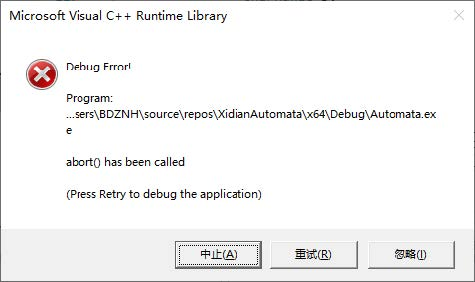
\includegraphics[width=0.60\textwidth]{DFA_usefulf_error}
    \caption{函数 DFA::usefulf() 错误提示}
    \label{fig::usefulf_error}
\end{figure}
控制台提示如图 \ref{fig::usefulf_console_log}
\begin{figure}[!htbp]
    \centering
    %trim option's parameter order: left bottom right top
    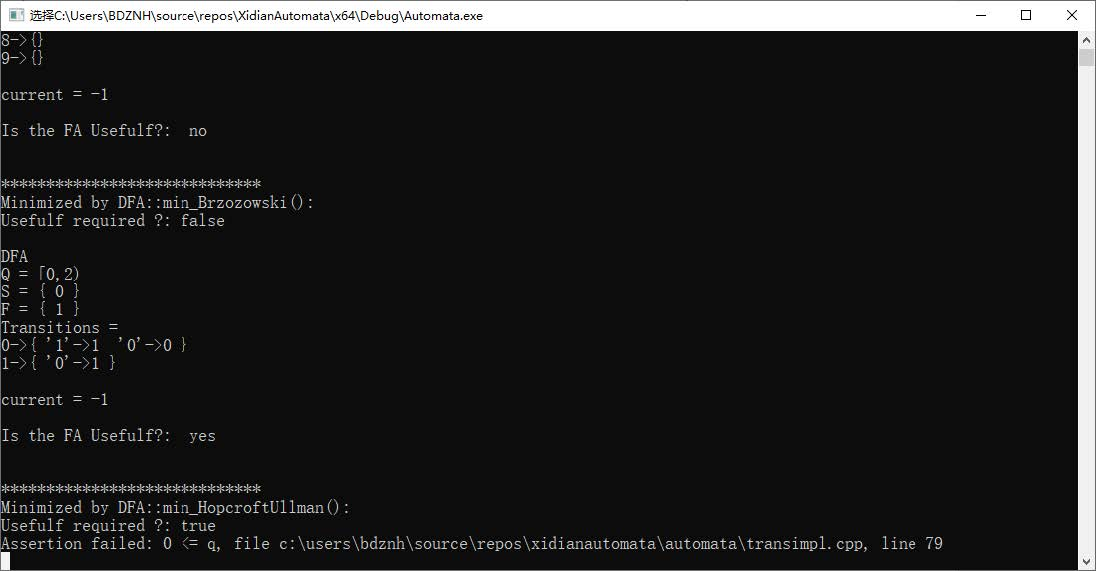
\includegraphics[trim = 0mm 0mm 0mm 63mm, clip,width=0.95\textwidth]{DFA_usefulf_console_log}
    \caption{函数 DFA::usefulf() 错误提示}
    \label{fig::usefulf_console_log}
\end{figure}

可以确定函数未完成其定义功能。

%%%%%%%%%%%%%%%%%%%%%%%%%%%%%%%%%%%%%%%%%%%%%%%%%%%%%%%%%%%%%%%%%%%%%%%%%%%%%%%%%%%%%%%%%%%%%%%%%%%%%%%%%%%%%%%%%%%%%%%%%%%%%%%%%%%%%%%%%%%%%%%%%%%%%%%%%%%%%%%%%%%%%%%%%%%%%
% {\bfseries 错误原因}
\subsection{错误原因}

查看 TransImple.cpp,79行,代码如下
\lstset{style=mystyle}
\begin{lstlisting}[language=C++,label={lst:TransImple},caption={ TransImple.cpp },firstnumber=75]
// Add a transition to the set.
TransImpl& TransImpl::add_transition(const CharRange a, const State q)
{
    assert(a.class_invariant());
    assert(0 <= q);
    ………
}
\end{lstlisting}

在 79 行处打断点,单步调试至此处,可以看到 State 变量 q 的值为“-842150451”,对应的十六进制值为“0xFFFFFFFF”\footnote{调试时使用 64 位编译器产生的二进制文件,在 64 位系统下运行。},为常见的未初始化错误。此时表达式 “0 <= q” 不成立,返回值为 “false” , 程序在此处中止。

查看函数 DFA::usefulf() 的实现,如代码 \ref{lst:DFA_usefulf_1} 。
\lstset{style=mystyle}
\begin{lstlisting}[language=C++,label={lst:DFA_usefulf_1},caption={ DFA.cpp },firstnumber=84]
StateTo<State> newnames;
newnames.set_domain(Q.size());

// All components will be constructed into a special structure :
DFA_components ret;
State st;
for (st = 0; st < Q.size(); st++)
{
    // If this is a Usefulf State, carry it over by giving it a name
    // in the new DFA.
    if (freachable.contains(st))
    {
        newnames.map(st) = ret.Q.allocate();
    }
}
\end{lstlisting}
在代码 \ref{lst:DFA_usefulf_1} 中将 “ final-reachable ” 状态保存到 StateTo<State> 变量 newnames 中,通过 “ ret.Q.allocate()” 为状态命名新的状态名,作为新的自动机的状态名。DFA\_components 变量 ret 用于构建新的自动机,再看函数内构造新的自动机的主要实现部分,如代码 \ref{lst:DFA_usefulf_2}
\lstset{style=mystyle}
\begin{lstlisting}[language=C++,label={lst:DFA_usefulf_2},caption={ DFA.cpp },firstnumber=130]
for (it = 0; !a.iter_end(it); it++)
{
    b = a.iterator(it);
    ret.T.add_transition(stprime, b, newnames.lookup(T.transition_on_range(st, b)));
}
\end{lstlisting}

根据代码 \ref{lst:TransImple} ,可以知道程序中止的地方为代码 \ref{lst:DFA_usefulf_2},133 行。其中 State 变量为当前需要进行操作的状态,CharRange 变量 b 为当前状态转移输入字符。查看 T.
transition\_on\_range(st, b)) 的实现,如代码 \ref{lst:transition_on_range}
\lstset{style=mystyle}
\begin{lstlisting}[language=C++,label={lst:transition_on_range},caption={ DTransRel.cpp },firstnumber=108]
// Compute the image of r, and CharRange it under *this.
inline State DTransRel::transition_on_range(const State r, const CharRange a) const
{
    assert(class_invariant());
    assert(0 <= r && r < domain());
    return(lookup(r).range_transition(a));
}
\end{lstlisting}
由代码 \ref{lst:transition_on_range} 可知,T.transition\_on\_range(st, b)) 将返回原自动机中,状态 st 经过输入字符 b 转移之后的目标状态。

查看 newnames.lookup() 的实现,如代码 \ref{lst:newnames-lookup}
\lstset{style=mystyle}
\begin{lstlisting}[language=C++,label={lst:newnames-lookup},caption={ StateTo.h },firstnumber=177]
// The actual mapping function
// First, a const lookup operator.
template<class T>
inline const T& StateTo<T>::lookup(const State r) const
{
    assert(class_invariant());
    // First check that it's in bounds
    assert(0 <= r && r < domain());
    return(data[r]);
}
\end{lstlisting}
在本例中,模板类 StateTo<T> 的模板参数 “T” 为 State。则 newnames.lookup(T.transition\_on\_range(st, b)) 为原自动机中 状态 st 经过字符 b 转移后的目标状态在新自动机中的状态。然后通过 ret.T.add\_transition() 保存新的转移关系。对所有的状态进行以上操作之后,通过变量 ret 构造新的自动机。 

经过单步调试发现,表\ref{tab:DFA4} 中,状态 $q_2$ 经过字符 “1” 将转移到状态 $q_5$,而在代码 \ref{lst:DFA_usefulf_1} 中,状态 $q_5$ 不满足 “if (freachable.contains(st))”,所以状态 $q_5$ 未被新的自动机保存,进而在代码 \ref{lst:DFA_usefulf_2} 中,当 st 为状态 $q_2$ 且 b 为字符 “1” 时,“newnames.lookup(T.transition\_on\_range(st, b))” 将返回未经初始化的值“-842150451”,于是在代码 \ref{lst:TransImple} 中,State 变量 q 的值为“-842150451”,导致程序在此处中止。

%%%%%%%%%%%%%%%%%%%%%%%%%%%%%%%%%%%%%%%%%%%%%%%%%%%%%%%%%%%%%%%%%%%%%%%%%%%%%%%%%%%%%%%%%%%%%%%%%%%%%%%%%%%%%%%%%%%%%%%%
\subsection{解决方法}

如代码 \ref{lst:State_H} 所示,文件 State.h 中将无效状态设置为 “Invalid”。在代码 \ref{lst:DFA_usefulf_1}增加处理不满足条件 “freachable.contains(st)” 的状态的内容,将原自动机中的非“final-reachable”状态标记为 “Invalid”,更改后为代码 \ref{lst:DFA_usefulf_1_edit}
\lstset{style=mystyle}
\begin{lstlisting}[language=C++,label={lst:DFA_usefulf_1_edit},caption={ 更改后的 DFA.cpp },firstnumber=91]
for (st = 0; st < Q.size(); st++)
{
    // If this is a Usefulf State, carry it over by giving it a name
    // in the new DFA.
    if (freachable.contains(st))
    {
        newnames.map(st) = ret.Q.allocate();
    }
    else                            // 新增
    {                               // 新增
        newnames.map(st) = Invalid; // 新增
    }                               // 新增
}
\end{lstlisting}

在代码 \ref{lst:DFA_usefulf_2} 中,在添加新的转移关系之前判断当前状态和目标状态是否都是有效状态,若都为有效状态,则添加新的转移关系。更改后为代码 \ref{lst:DFA_usefulf_2_edit}
\lstset{style=mystyle}
\begin{lstlisting}[language=C++,label={lst:DFA_usefulf_2_edit},caption={ 更改后的 DFA.cpp },firstnumber=133]
    State stdest;                                           // 新增
    stdest = newnames.lookup(T.transition_on_range(st, b)); // 新增

    if (stprime != Invalid &&  stdest != Invalid)           // 新增
    {                                                       // 新增
        ret.T.add_transition(stprime, b, stdest));          // 修改
    }                                                       // 新增
\end{lstlisting}

更改后函数 DFA::usefulf() 成功移除图 \ref{fig:DFA4_0} 中的陷阱状态 $q_5$ ,将图 \ref{fig:DFA4_0} 转换成图 \ref{fig:DFA4_1}。
更改后函数 DFA::usefulf() 成功移除图 \ref{fig:usefulf2-1} 中的陷阱状态 $q_1$ ,将图 \ref{fig:usefulf2-1} 转换成图 \ref{fig:usefulf2-2} 。



%%%%%%%%%%%%%%%%%%%%%%%%%%%%%%%%%%%%%%%%%%%%%%%%%%%%%%%%%%%%%%%%%%%%%%%%%%%%%%%%%%%%%%%%%%%%%%%%%%%%%%%%%%%%%%%%%%%%%%%%%%%%%%%%%%%%%%%%%%%%%%%%%%%%%%%%%%
%%%%%%%%%%%%%%%%%%%%%%%%%%%%%%%%%%%%%%%%%%%%%%%%%%%%%%%%%%%%%%%%%%%%%%%%%%%%%%%%%%%%%%%%%%%%%%%%%%%%%%%%%%%%%%%%%%%%%%%%%%%%%%%%%%%%%%%%%%%%%%%%%%%%%%%%%%
\section{函数 DFA::min\_Hopcroft() 运行错误}\label{sec:hopcroft}

% Hopcroft 算法描述如下\cite{watson1993taxonomyb} \\
% {\small \setlength{\parskip}{1em}
% \rule{\textwidth}{1pt}
% \mbox{ } $P:=[Q]_{E_0}$; \\
% \mbox{ } $L:= ( \mbox{\textbf{if }} ( |F| \leq |Q \setminus F | ) \mbox{\textbf{then }} \{F\} \mbox{\textbf{else }} \{ Q \setminus F \} \mbox{\textbf{fi }} ) \times V $; \\
% \mbox{ } $ \{ \mbox{恒有: } [Q]_E \sqsubseteq P \sqsubseteq [Q]_{E_0} \land L \subseteq (P \times V) $ \\
% \mbox{   } $ \land (\forall Q_0,Q_1,a:Q_0 \in Q \land (Q_1,a) \in L : \neg Splittable (Q_0,Q_1,a)) \Rightarrow (P=[Q]_E) \} $ \\
% \mbox{ } $ \mbox{\textbf{do }} L \not= \emptyset \longrightarrow $ \\ 
% \mbox{   } $ \mbox{\textbf{let }} Q_1,a:(Q_1,a) \in L $; \\
% \mbox{   } $ P_{old} := P $; \\
% \mbox{   } $ L := L \setminus \{ (Q_1,a) \} $; \\
% \mbox{   } $ \{  \mbox{恒有: } [Q]_E \sqsubseteq P \sqsubseteq P_{old} \} $ \\
% \mbox{   } $ \mbox{\textbf{for }} Q_0 : Q_0 \in P_{old} \land Splittable (Q_0,Q_1,a) \mbox{\textbf{ do }} $ \\
% \mbox{     } $ Q'_0 := \{ p:p \in Q_0 \land T(p,a) \in Q_1 \} $; \\
% \mbox{     } $ P:= P \setminus \{ Q_0 \} \cup \{ Q_0 \setminus Q'_0,b \} $;\\
% \mbox{     } $ \mbox{\textbf{for }} b:b \in V \mbox{\textbf{ do }} $ \\
% \mbox{       } $ \mbox{\textbf{if }} (Q_0,b) \in L \rightarrow L := L \setminus \{ (Q_0,b) \} \cup \{ (Q'_0,b),(Q_0, \setminus Q'_0,b ) \} $;\\ 
% \mbox{       } $ \talloblong (Q_0,b) \notin L \rightarrow $ \\
% \mbox{         } $ L := L \cup (\mbox{\bfseries if} ( |Q'_0| \leq |Q_0 \setminus Q'_0| ) \mbox{\bfseries then} \{ (Q'_0 , b) \} \mbox{\bfseries else} \{ ( Q'_0 \setminus Q'_0,b ) \} \mbox{\bfseries fi} ) $ \\
% \mbox{       } $ \mbox{\textbf{fi}} $ \\
% \mbox{     } $ \mbox{\textbf{rof}} $ \\
% \mbox{   } $ \mbox{\textbf{rof}} $ \\
% \mbox{   } $ \{ (\forall Q_0,Q_0 \in P : \neg Splittable(Q_0,Q_1,a)) \} $ \\
% \mbox{ } $ \mbox{\textbf{od }} \{ P = [Q]_E \} $ \\
% \rule{\textwidth}{1pt} }

实例化如表 \ref{tab:DFA411-1} 所示的自动机。(含有开始不可达状态\footnote{从开始状态不可以到达的状态,如图 \ref{fig:DFA11-0} 中状态 $q_9$ 。}(start-unreachable))

\begin{table}[!htbp]
    \caption{图\ref{fig:DFA11-0}的转移函数}
    \label{tab:DFA411-1}
    \centering
    \small% fontsize
    \setlength{\tabcolsep}{4pt}% column separation
    \renewcommand{\arraystretch}{1.2}%row space 
    %\begin{tabular}{lcrr} 
        \begin{tabular}{l p{4em}<{\centering} p{3em}<{\centering} p{3em}<{\centering}}
        \toprule %\hline 
        \multirow{2}{*}{状态说明} & \multirow{2}{*}{状态} & \multicolumn{2}{c}{输入字符} \\
		\cline{3-4}      &    &$0$ & $1$  \\
        \midrule%\hline
        开始状态(start)  & $q_0$ & $q_1$   & $q_2$   \\
                        & $q_1$ & $q_5$   & $q_2$   \\
                        & $q_2$ & $q_3$   & $q_6$   \\
                        & $q_3$ & $q_2$   & $q_4$   \\
        结束状态(final) & $q_4$ & $q_8$   & $q_1$   \\
                        & $q_5$ & $q_1$   & $q_6$   \\
                        & $q_6$ & $q_7$   & $q_2$   \\
                        & $q_7$ & $q_6$   & $q_8$   \\
        结束状态(final) & $q_8$ & $q_5$   & $q_4$   \\
        开始不可达状态    & $q_9$ & $q_7$   & $q_5$   \\
        \bottomrule%\hline 
    \end{tabular}
\end{table}

函数 DFA::min\_Hopcroft() 是 Hopcroft 算法在 FIRE engine 中的实现,Hopcroft 算法在文中\cite{watson1993taxonomyb}描述如下:
\begin{figure}[!htbp]
    \centering
        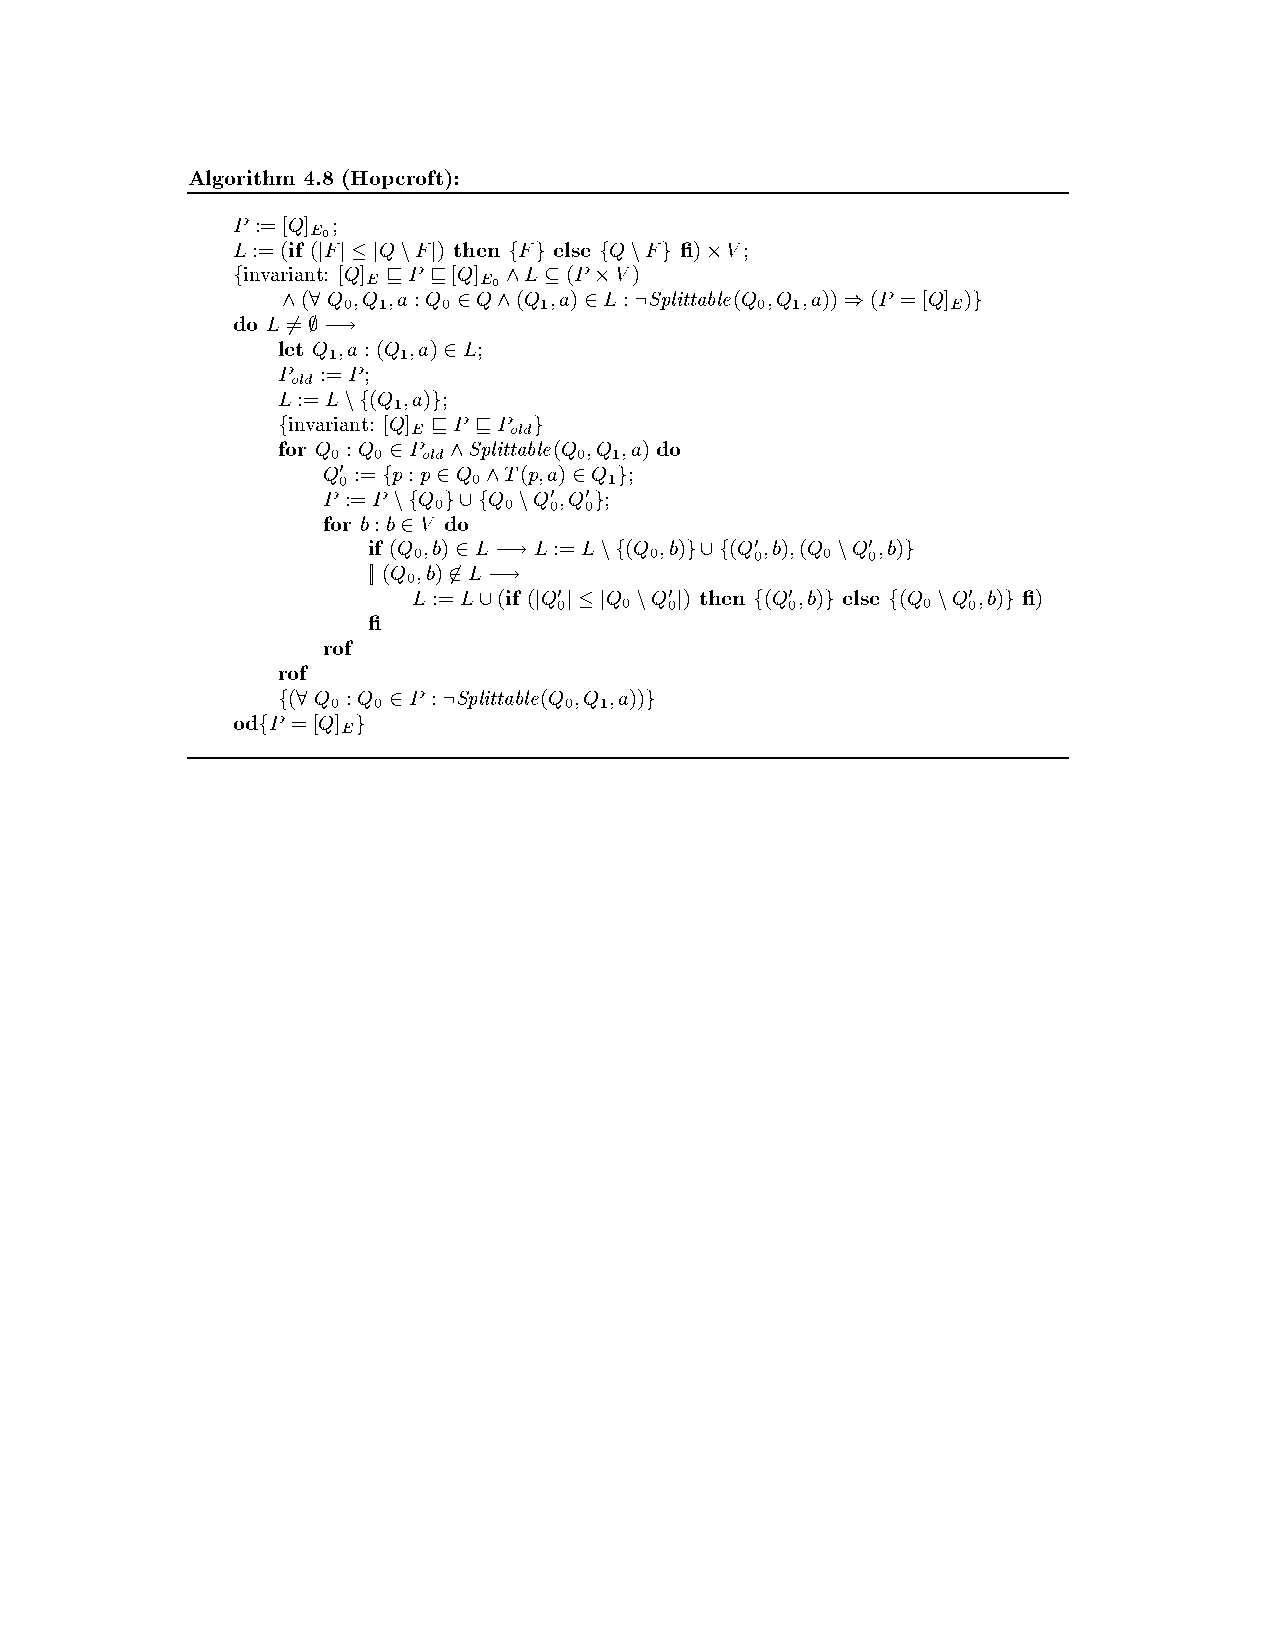
\includegraphics[width=0.99\textwidth]{hopcroft}
\end{figure}

\subsection{运行结果}\label{sec:hopcroft-error}
执行函数 DFA::min\_Hopcroft(),程序在文件CRSet.h,第 146 行的 “assert(!iter\_end(it))” 处触发 assert 中止,如代码 \ref{lst:iterend} 所示。调用函数“CRSet::iterator()”的地方为文件min-hop.cpp,第103行,“State r(split(p, q, C.iterator(L[q]), P));”的“C.iterator(L[q])”处。
\lstset{style=mystyle}
\begin{lstlisting}[language=C++,label={lst:iterend},caption={ CRSet.h },firstnumber=142]
// Fetch the it'th CharRange in *this.
inline const CharRange& CRSet::iterator(const int it) const
{
    assert(class_invariant());
    assert(!iter_end(it));
    return(data[it]);
}

// Is there even in it'th CharRange?
inline int CRSet::iter_end(const int it) const
{
    assert(class_invariant());
    assert(0 <= it);
    return(it >= in_use);
}
\end{lstlisting}

\subsection{错误原因}

以表 \ref{tab:DFA411-1} 中实例化的自动机为例,CRSet 变量 C = \{ 0, 1\},在程序中止处打断点,调试至此处可看到 int 变量 it 为 “2”,因 C 中只有两个值 “1、2”,所以传入参数为 “2” 时,超出可以 C 的范围,于是在语句 “assert(!iter\_end(it));” 处导致程序中止。

算法迭代过程如附录表 \ref{tab:hopcroft} 所示。

在第 11 次迭代中,DFA::split() 函数将等价类\{0,1,5\} 分割为等价类 \{\{0\},\{1,5\}\},此时$p=0,q=0,r=1$,满足条件$|Q'_0| \leq | Q_0 \setminus Q'_0 |$,执行 L[r] = L[p] =1,L[p] = C.size() = 2。在第 12 次迭代中,由于第 11 次迭代中 $p=q$ ,所以 L[q] 的值将被更改为 “2”,于是在 C.iterator(L[q]) 处传入一个超过 C 的范围的值,程序触发 assert 中止。

\subsection{解决方法}

函数 DFA::min\_Hopcroft() 的主要实现部分如代码 \ref{lst:hopcroft-iter}。
\lstset{style=mystyle}
\begin{lstlisting}[language=C++,label={lst:hopcroft-iter},caption={ min-hop.cpp },firstnumber=100]
    for (repr.iter_start(p); !repr.iter_end(p); repr.iter_next(p))
    {
        //分割等价类
        ……
    }
\end{lstlisting}

在分割等价类之前,判断 L[q] 是否等于 “C.size()”,若是,则减去 “1”,更改后为代码 \ref{lst:hopcroft-iter-edit}

\lstset{style=mystyle}
\begin{lstlisting}[language=C++,label={lst:hopcroft-iter-edit},caption={ min-hop.cpp },firstnumber=100]
    for (repr.iter_start(p); !repr.iter_end(p); repr.iter_next(p))
    {
        if(L[q] == C.size()) // 新增
        {                    // 新增
            L[q]--;          // 新增
        }                    // 新增
        //分割等价类
        ……
    }
\end{lstlisting}

更改后函数 DFA::min\_Hopcroft() 运行不再中止。

%%%%%%%%%%%%%%%%%%%%%%%%%%%%%%%%%%%%%%%%%%%%%%%%%%%%%%%%%%%%%%%%%%%%%%%%%%%%%%%%%%%%%%%%%%%%%%%%%%%%%%%%%%%%%%%%%%%%%%%%%%%%%%%%
%%%%%%%%%%%%%%%%%%%%%%%%%%%%%%%%%%%%%%%%%%%%%%%%%%%%%%%%%%%%%%%%%%%%%%%%%%%%%%%%%%%%%%%%%%%%%%%%%%%%%%%%%%%%%%%%%%%%%%%%%%%%%%%%
\section{测试结果汇总}

经过 \ref{sec:ohloop} 节、\ref{sec:usefulf} 节和 \ref{sec:hopcroft} 节的修改,FIRE engine 中的最小化算法及最小化算法用到的帮助函数都可以成功运行。本节内容为测试正确的结果和一些未能解决的问题的汇总。

\subsection{不改变已经是最小的 DFA 接受的语言}

接受一个 $\mathcal{L}$ 的最小的 DFA 是唯一的,最小的且接受相同 $\mathcal{L}$ 的 DFA 仅仅在状态命名上有差别\cite{book1}。因此最小化算法有性质 \ref{sec:keepMin} 。

\begin{property}\label{sec:keepMin}
    由定义 \ref{def:min} 可知,对于 DFA $M$,$\mathcal{L}(Min(M))= \mathcal{L}(M)$,同样的,最小化算法不能使最小的 DFA 接受的 $\mathcal{L}$ 发生改变。
\end{property}

\begin{remark}
    DFA 中的 开始不可达(start-unreachable)状态和陷阱状态(final-unreachable)状态不影响 DFA 接受的 $\mathcal{L}$。
\end{remark}



\begin{table}[!htbp]
    \caption{一组最小的 DFA}
    \label{tab:KeepMinData}
    \centering
    \small% fontsize
    \setlength{\tabcolsep}{4pt}% column separation
    \renewcommand{\arraystretch}{1.2}%row space 
    \begin{tabular}{c p{4em}<{\centering} p{4em}<{\centering} l}  %l p{3em}<{\centering} p{3em}<{\centering} p{3em}<{\centering}
        \toprule %\hline 
                序号  &  数据 & 属性 & 备注 \\
        \midrule%\hline
        1 &  图 \ref{fig:usefulf2-1} & 最小的 & 含有陷阱状态 \\
        2 &  图 \ref{fig:usefulf2-2} & 最小的 & 不含陷阱状态 \\
        \midrule
        3 & 图 \ref{fig:DFA11-0} & 最小的 & 含有开始不可达状态 \\
        4 & 图 \ref{fig:DFA11-1} & 最小的 & 不含开始不可达状态 \\
       \midrule
        5 & 图 \ref{fig:keepMin-1-unreachable} & 最小的 & 含有开始不可达状态 \\
        6 & 图 \ref{fig:keepMin-1-nonTheState} & 最小的 & 不含开始不可达状态 \\
       \midrule
        7 & 图 \ref{fig:keepMin-2-unreachable} & 最小的 & 含有开始不可达状态 \\
        8 & 图 \ref{fig:keepMin-2-nonTheState} & 最小的 & 不含开始不可达状态 \\
        \bottomrule%\hline  
    \end{tabular}
\end{table}


对于性质 \ref{sec:keepMin} ,以表 \ref{tab:KeepMinData} 中的一组最小的 DFA 为数据,测试结果表 \ref{tab:KeepMinResult} 所示。




\begin{table}[!htbp]
    \caption{ 最小化算法对性质 \ref{sec:keepMin} 的测试结果 }
    \label{tab:KeepMinResult}
    \centering
    \small% fontsize
    \setlength{\tabcolsep}{4pt}% column separation
    \renewcommand{\arraystretch}{1.2}%row space 
    \begin{tabular}{l|p{2em}<{\centering} p{2em}<{\centering} p{2em}<{\centering} p{2em}<{\centering} p{2em}<{\centering} p{2em}<{\centering} p{2em}<{\centering} p{2em}<{\centering}}  %l p{3em}<{\centering} p{3em}<{\centering} p{3em}<{\centering}
        \toprule %\hline 
        算法 & 1 & 2 & 3 & 4 &  5 &  6  & 7 & 8  \\
        \midrule
        DFA::min\_Brzozowski()        & $\surd$ & $\surd$ & $\times$  & $\times$  & $\checkmark$ & $\surd$ & $\checkmark$ & $\surd$ \\
        DFA::min\_Hopcroft()(修改前) & $\surd$ & $\surd$ & 中止    & $\surd$     & $\surd$ & $\surd$ & $\surd$ & $\surd$ \\
        DFA::min\_Hopcroft()(修改后) & $\surd$ & $\surd$ & $\surd$ & $\surd$     & $\surd$ & $\surd$ & $\surd$ & $\surd$ \\
        DFA::min\_HopcroftUllman()    & $\surd$ & $\surd$ & $\surd$ & $\surd$     & $\surd$ & $\surd$ & $\surd$ & $\surd$ \\
        DFA::min\_dragon()            & $\surd$ & $\surd$ & $\surd$ & $\surd$     & $\surd$ & $\surd$ & $\surd$ & $\surd$ \\
        DFA::min\_Watson()            & $\surd$ & $\surd$ & $\surd$ & $\surd$     & $\surd$ & $\surd$ & $\surd$ & $\surd$ \\
        \bottomrule%\hline  
    \end{tabular}
\end{table}

对表 \ref{tab:KeepMinResult} 中的测试结果有两个算法需要额外关注—— “DFA::min\_Brzozowski()” 和 “DFA::min\_Hopcroft()”。

结果总结对比如下:
\begin{itemize}
    \item 对于 DFA 中的陷阱状态,可以调用函数 “DFA::usefulf()” 函数去除。表 \ref{tab:KeepMinResult} 中在执行最小化函数之前,除了算法 “DFA::min\_Brzozowski”, 都执行了函数 “DFA::usefulf()”;
    \item 除了算法 “DFA::min\_Brzozowski()” 外,其他最小化算法均不能去除 DFA 中的开始不可达状态(start-unreachable)。数据为第 5 个和第 7 个,以 $\checkmark$ 标示,而不是 $\surd$;
    \item 对于算法 “DFA::min\_Hopcroft()” 的 assert 中止,在发生 assert 中止的第 3 个数据中,含有开始不可达状态,作为对照组且含有开始不可达状态的第 5 个和第 7 个数据确没有发生 assert 中止,所以本文认为此算法的中止的问题不是 DFA 中开始不可达状态导致;
    \item 对于第 3 个和第 4 个数据,算法 “DFA::min\_Brzozowski()” 改变了 DFA ,输入的 DFA 仅有 10/9 个状态,算法 “DFA::min\_Brzozowski()” 输出了含有数百个状态的自动机。
\end{itemize}



\subsection{最小化功能测试}

本节内容为最小化算法对定义功能的测试,以表 \ref{tab:MinData} 中的数据对五个最小化算法进行测试,结果如表 \ref{tab:MinResult} 所示。

\begin{table}[!htbp]
    \caption{一组 DFA}
    \label{tab:MinData}
    \centering
    \small% fontsize
    \setlength{\tabcolsep}{4pt}% column separation
    \renewcommand{\arraystretch}{1.2}%row space 
    \begin{tabular}{c p{4em}<{\centering} p{4em}<{\centering} c }  %l p{3em}<{\centering} p{3em}<{\centering} p{3em}<{\centering}
        \toprule %\hline 
                序号  &  数据 & 属性 & 预期结果  \\
        \midrule%\hline
        1 &  图 \ref{fig:DFA4_0} &            & 图 \ref{fig:DFA4_3}\\
        \midrule
        2 & 图 \ref{fig:DFAMin-3-0} &         & 图 \ref{fig:DFAMin-3-2}  \\
        3 & 图 \ref{fig:DFAMin-3-1} & 最小的  & 图 \ref{fig:DFAMin-3-1}  \\
        \midrule
        4 & 图 \ref{fig:DFAMin-5-0} &         & 图 \ref{fig:DFAMin-5-2}  \\
        5 & 图 \ref{fig:DFAMin-5-1} & 最小的  & 图 \ref{fig:DFAMin-5-1}  \\
        \midrule
        6 & 图 \ref{fig:DFAMin-4-0} &        & 图 \ref{fig:DFAMin-4-2}  \\
        7 & 图 \ref{fig:DFAMin-4-1} & 最小的  & 图 \ref{fig:DFAMin-4-1}  \\
        \bottomrule%\hline  
    \end{tabular}
\end{table}

\begin{table}[!htbp]
    \caption{ 最小化算法的定义功能的测试结果 }
    \label{tab:MinResult}
    \centering
    \small% fontsize
    \setlength{\tabcolsep}{4pt}% column separation 
    \renewcommand{\arraystretch}{1.2}%row space 
    \begin{tabular}{l| p{2em}<{\centering} p{2em}<{\centering} p{2em}<{\centering} p{2em}<{\centering} p{2em}<{\centering} p{2em}<{\centering} p{2em}<{\centering} }  %l p{3em}<{\centering} p{3em}<{\centering} p{3em}<{\centering}
        \toprule %\hline 
        算法 & 1 & 2 & 3 & 4 &  5 & 6 & 7 \\
        \midrule
        DFA::min\_Brzozowski()        & $\surd$ & $\surd$ & $\surd$   & $\surd$ & $\surd$ & $\surd$     & $\surd$       \\
        DFA::min\_Hopcroft()(修改前) & $\surd$ & $\surd$ & $\times$  & $\surd$ & $\surd$ & 中止        & $\surd$       \\
        DFA::min\_Hopcroft()(修改后) & $\surd$ & $\surd$ & $\times$  & $\surd$ & $\surd$ & $\surd$     & $\surd$       \\
        DFA::min\_HopcroftUllman()    & $\surd$ & $\surd$ & $\surd$   & $\surd$ & $\surd$ & $\surd$     & $\surd$       \\
        DFA::min\_dragon()            & $\surd$ & $\surd$ & $\surd$   & $\surd$ & $\surd$ & $\surd$     & $\surd$       \\
        DFA::min\_Watson()            & $\surd$ & $\surd$ & $\surd$   & $\surd$ & $\surd$ & $\surd$     & $\surd$       \\
        \bottomrule%\hline  
    \end{tabular}
\end{table}

对于第 3 个数据,算法 “DFA::min\_Hopcroft()” 无论是否经过第 \ref{sec:hopcroft} 节的修改,均输出代码 \ref{lst:hoperrorResult} 。
\lstset{style=mystyle}
\begin{lstlisting}[language=C++,label={lst:hoperrorResult},caption={ 第 3 个数据在算法 “DFA::min\_Hopcroft()” 中的输出 }]
DFA
Q = [0,2)
S = { 0 }
F = { 1 }
Transitions =
0->{ ['a','b']->1 }
1->{ 'a'->1 }

current = -1
\end{lstlisting}

第 3 个数据的转移函数如表 \ref{tab:sample_3_origin} 所示 ,代码 \ref{lst:hoperrorResult} 的转移函数如表 \ref{tab:sample_3_result} 所示 

% \begin{table}[!htbp]
%     \caption{接受{$\mathcal{L}=0^*10^*$}的自动机{\cite{book1}}}
%     \label{tab:hopcroftErrorResult}
%     \centering
%     \small% fontsize
%     \setlength{\tabcolsep}{4pt}% column separation
%     \renewcommand{\arraystretch}{1.2}%row space 
%     %\begin{tabular}{lcrr} 
%         \begin{tabular}{l p{3em}<{\centering} p{3em}<{\centering} p{3em}<{\centering}}
%         \toprule %\hline 
%         \multirow{2}{*}{状态说明} & \multirow{2}{*}{状态} & \multicolumn{2}{c}{输入字符} \\
% 		\cline{3-4}      &    &$0$ & $1$  \\
%         \midrule%\hline
%         开始状态(start)  & $q_0$ & $q_1$   & $q_2$   \\
%                         & $q_1$ & $q_0$   & $q_3$   \\
%         结束状态(accept) & $q_2$ & $q_4$   & $q_5$   \\
%         结束状态(accept) & $q_3$ & $q_4$   & $q_5$   \\
%         结束状态(accept) & $q_4$ & $q_4$   & $q_5$   \\
%         陷阱状态(sink) & $q_5$ & $q_5$   & $q_5$   \\
%         \bottomrule%\hline 
%     \end{tabular}
% \end{table}

\begin{table}[!htbp]
    \caption{第 3 个数据在算法 “DFA::min\_Hopcroft()” 中的输入输出对比 }
    \label{tab:sample_3}
    \centering
    \small% fontsize
    \setlength{\tabcolsep}{4pt}% column separation
    \renewcommand{\arraystretch}{1.2}%row space 
    \begin{subtable}[t]{0.45\textwidth}
        \centering
        \caption{输入}
        \label{tab:sample_3_origin}
        \begin{tabular}{l p{2em}<{\centering} c c}
            \toprule%\hline
            \multirow{2}{*}{状态说明} & \multirow{2}{*}{状态} & \multicolumn{2}{c}{输入字符} \\
            \cline{3-4}      &    &$a$ & $b$  \\
            %\cline{2-9}% partial hline from column i to column j
            \midrule%\hline
            开始状态(start)  & $q_0$ & $q_1$   & $q_2$   \\
            结束状态(final) & $q_1$ & $q_2$   &     -   \\
            结束状态(final) & $q_2$ & -       & $q_1$   \\
            \bottomrule%\hline
        \end{tabular}
    \end{subtable}
    ~% add desired spacing
    \begin{subtable}[t]{0.45\textwidth}
        \centering
        \caption{输出}
        \label{tab:sample_3_result}
        \begin{tabular}{l p{2em}<{\centering} c c }
            \toprule%\hline
            \multirow{2}{*}{状态说明} & \multirow{2}{*}{状态} & \multicolumn{2}{c}{输入字符} \\
            \cline{3-4}      &    & $a$ & $b$  \\
            %\cline{2-9}% partial hline from column i to column j
            \midrule%\hline
            开始状态(start)  & $q_0$ & $q_1$   & $q_1$   \\
            结束状态(final) & $q_1$ & $q_1$   & -   \\
            & & & \\
            \bottomrule%\hline
        \end{tabular}
    \end{subtable}
\end{table}

图 \ref{fig:DFAMin-3-1} 原本是一个最小的 DFA,由表 \ref{tab:sample_3} 可知,函数算法 “DFA::min\_Hopcroft()” 已经改变了图 \ref{fig:DFAMin-3-1} 的状态数,由 “3” 变到 “2”, 如图 \ref{fig:DFAMinHoop-3} 所示,已经不满足性质 \ref{sec:keepMin}。由此可以认为 FIRE engine 中算法 “DFA::min\_Hopcroft()” 未完成其定义功能。

\begin{figure}[!htbp]
    \centering
    \begin{subfigure}[b]{0.4\textwidth}
        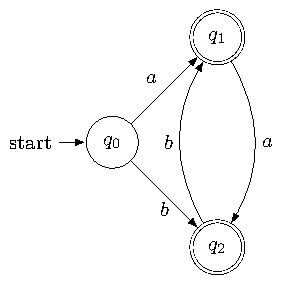
\includegraphics[width=\textwidth]{Min/DFAMinTest-3-1}
        \caption{输入}
        \label{fig:DFAMin-3-1-inside}
    \end{subfigure}
    ~
    \begin{subfigure}[b]{0.4\textwidth}
        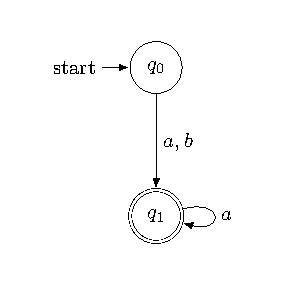
\includegraphics[width=\textwidth]{Min/DFAMinTest-3-3}
        \caption{输出}
        \label{fig:DFAMin-3-3-inside}
    \end{subfigure}
    \caption{DFA::min\_Hopcroft 对第 3 个数据输入输出对比}
    \label{fig:DFAMinHoop-3}
  \end{figure}

对于算法 “DFA::min\_Hopcroft()” 和算法 “DFA::min\_Brzozowski” 的扩展测试见附录。